
\documentclass[11pt]{article}
\usepackage{amsmath,amsfonts,amssymb,amsthm}
\usepackage{mathpazo}
\usepackage{fullpage}
\usepackage{enumerate}

\usepackage{xcolor}

\def\naturals{\mathbb{N}}
\def\integers{\mathbb{Z}}
\def\rationals{\mathbb{Q}}
\def\reals{\mathbb{R}}
\def\complex{\mathbb{C}}
\renewcommand{\Im}{\operatorname{Im}}
\renewcommand{\Re}{\operatorname{Re}}
\newcommand{\abs}[1]{\left|#1\right|}

 \usepackage{hyperref}
\hypersetup{
  colorlinks   = true, %Colours links instead of ugly boxes
  urlcolor     = blue, %Colour for external hyperlinks
  linkcolor    = blue, %Colour of internal links
  citecolor   = red %Colour of citations
}
\usepackage{tikz}
\usepackage{pgfplots}
\pgfplotsset{complexstyle/.append style={axis x line=middle, axis y line=
middle, xlabel={$\operatorname{Re}$}, ylabel={$\operatorname{Im}$}, axis equal ,every axis x label/.style={
    at={(ticklabel* cs:1.0)},
    anchor=west,
},
every axis y label/.style={
    at={(ticklabel* cs:1.0)},
    anchor=south,
}}}


\usepackage[most]{tcolorbox}
\usepackage{environ}

\newif\ifshowsolution
\showsolutionfalse
\showsolutiontrue

\NewEnviron{Solution}{%
    \ifshowsolution%
        \begin{tcolorbox}[colback=white,colframe=gray!10,enhanced,breakable]%
            \textbf{Solution.} \BODY
        \end{tcolorbox}%
    \fi%
}%


\usepackage{textcomp}


  \usepackage{polynom}

\polyset{%
  style=A
  %div=:
}


\begin{document}

\title{MATH 135 --- Fall 2021\\ Practice Problems \ifshowsolution(Solutions)\fi -- Chapters 9 and 10}
\author{Mark Girard}
\date{December 3, 2021}

\maketitle

Topics: Complex numbers and polynomials.
 
\begin{enumerate}%\itemsep0em 
 \item Express the following complex numbers in \textbf{standard form}. (That is, find $x,y\in\reals$ such that $z=x+yi$.)
 
  \begin{enumerate}
   \item $\displaystyle\frac{1+i}{1-i}$
   \begin{Solution}
    Note that we can multiply the top and bottom by the conjugate of $1-i$ to find
    \[
     \frac{1+i}{1-i} = \frac{1+i}{1-i}\frac{1+i}{1+i} = \frac{(1+i)^2}{|1+i|^2} = \frac{(1-1) + i(1+1)}{1^2 + 1^2} = \frac{0+2i}{2} = i.
    \]
\begin{center}
    \begin{tikzpicture}[scale=.80,every node/.style={scale=0.8}]
   \draw[<->] (-5/2,0) -- (5/2,0) node[right] {$\text{Re}$};
   \draw[<->] (0,-5/2) -- (0,5/2) node[above] {$\text{Im}$};
   \filldraw [red] (0,1) circle (2pt) node[left, black] {$i$};
\end{tikzpicture}
\end{center}
   \end{Solution}


   \item $\displaystyle\frac{3+i}{2-5i}$
\begin{Solution}
    Note that we can multiply the top and bottom by the conjugate of $2-5i$ to find
    \begin{multline*}
    \frac{3+i}{2-5i} = \frac{3+i}{2-5i}\frac{2+5i}{2+5i} = \frac{(3+i)(2+5i)}{|2-5i|^2} \\= \frac{(3\cdot 2 - 1\cdot 5) + i(3\cdot 5 + 1\cdot 2)}{2^2 + 5^2} = \frac{(6-5)+i(15+2)}{4+25} = \frac{1}{29} + \frac{17}{29}i.
    \end{multline*}
    \begin{center}
    \begin{tikzpicture}[scale=.80,every node/.style={scale=0.8}]
   \draw[<->] (-5/2,0) -- (5/2,0) node[right] {$\text{Re}$};
   \draw[<->] (0,-5/2) -- (0,5/2) node[above] {$\text{Im}$};
    \draw [dashed,gray] (.1,0) -- (.1,1);
   \draw [black] (-.1,1) -- (.1,1);
   \draw [black] (.1,-.1) -- (.1,.1);
   \filldraw [red] (0.1,1) circle (2pt) node[right, black] {$\frac{1}{29}+\frac{17}{29}i$};
\end{tikzpicture}
\end{center}


   \end{Solution}
   \item $\displaystyle\frac{(\sqrt{3}+i)^2}{(\sqrt{3}-i)(1+\sqrt{3}i)}$
   \begin{Solution}
Note that we can multiply out the denominator to find
\begin{align*}
 (\sqrt{3}-i)(1+\sqrt{3}i) = (\sqrt{3}+\sqrt{3}) + (3-1)i &= 2\sqrt{3} + 2i\\ &= 2(\sqrt{3}+i)
\end{align*}
and thus 
\begin{align*}
 \frac{(\sqrt{3}+i)^2}{(\sqrt{3}-i)(1+\sqrt{3}i)} &= \frac{(\sqrt{3}+i)^2}{2(\sqrt{3}+i)} \\
 &=\frac{\sqrt{3}+i}{2} = \frac{\sqrt{3}}{2} + \frac{1}{2}i.
\end{align*}
    \begin{center}
    \begin{tikzpicture}[scale=.80,every node/.style={scale=0.8}]
   \draw[<->] (-5/2,0) -- (5/2,0) node[right] {$\text{Re}$};
   \draw[<->] (0,-5/2) -- (0,5/2) node[above] {$\text{Im}$};
     \draw [dashed,gray] (1.73,0) -- (1.73,1);
     \draw [dashed,gray] (0,1) -- (1.73,1);
    \draw [black] (-.1,1) -- (.1,1);
    \draw [black] (1.73,-.1) -- (1.73,.1);
    \filldraw [red] (1.73,1) circle (2pt) node[above, black] {$\frac{\sqrt{3}}{2}+\frac{i}{2}$};
\end{tikzpicture}
\end{center}
\end{Solution}
   \item $(i-1)^4$
   \begin{Solution}
Note that $i-1$ can be expressed in polar form as
\[
 i-1 = \sqrt{2}\left(-\frac{1}{\sqrt{2}}+\frac{1}{\sqrt{2}}i\right) = \sqrt{2}\operatorname{cis}\left(\frac{3\pi}{4}\right),
\]
and thus 
\[
 (i-1)^4 = \sqrt{2}^4 \operatorname{cis}\left(\frac{3\pi}{4}\right)^4 = 4\operatorname{cis}\left(3\pi\right) = 4\bigl(\cos(3\pi)+i\sin(3\pi)) = 4(-1+0i) = -4,
\]
hence  $(i-1)^4=-4$
\begin{center}
    \begin{tikzpicture}[scale=.80,every node/.style={scale=0.8}]
   \draw[<->] (-5/2,0) -- (5/2,0) node[right] {$\text{Re}$};
   \draw[<->] (0,-5/2) -- (0,5/2) node[above] {$\text{Im}$};
     %\draw [dashed,gray] (1.73,0) -- (1.73,1);
     %\draw [dashed,gray] (0,1) -- (1.73,1);
    %\draw [black] (-.1,1) -- (.1,1);
    %\draw [black] (1.73,-.1) -- (1.73,.1);
    \filldraw [red] (-2,0) circle (2pt) node[above, black] {$-4$};
\end{tikzpicture}
\end{center}
\end{Solution}

 \end{enumerate}

\item Express the following complex numbers in \textbf{polar form}. (That is, find real numbers $r,\theta\in\reals$ such that $z=r(\cos\theta + i\sin\theta)$, $0\leq r$, and $0\leq\theta<2\pi$.)
 
  \begin{enumerate}
   \item $\displaystyle\frac{1+i}{1-i}$
   \begin{Solution}
    From 1a we have that $\frac{1+i}{1-i} = i$, which in polar form is \[i=\operatorname{cis}\left(\frac{\pi}{2}\right) = \cos \left(\frac{\pi}{2}\right)+i\sin \left(\frac{\pi}{2}\right).\]
   \begin{center}
    \begin{tikzpicture}[scale=.80,every node/.style={scale=0.8}]
   \draw[<->] (-5/2,0) -- (5/2,0) node[right] {$\text{Re}$};
   \draw[<->] (0,-5/2) -- (0,5/2) node[above] {$\text{Im}$};
    \draw[blue] (.5cm,0cm) arc (0:90:.5cm);
   \draw[blue,-,thick] (0,0) -- (0,1) ;
   \filldraw [red] (0,1) circle (2pt) node[left, black] {$i$} node[blue,below right] {$\frac{\pi}{2}$};
\end{tikzpicture}
\end{center}
   \end{Solution}


   \item $\displaystyle\frac{5+i}{2i-3}$
   \begin{Solution}
Note that 
\begin{align*}
 \frac{5+i}{2i-3} = \frac{5+i}{2i-3}\frac{-2i-3}{-2i-3} &= \frac{(5+i)(-2i-3)}{|2i-3|^2} \\&= \frac{(-15+2)+(-10-3)i}{2^2 + 3^2} \\&= \frac{13+13i}{4+9} \\&= \frac{13(1+i)}{13} = 1+i
\end{align*}
and in polar form this is
\[
 1+i = \sqrt{2}\left(\frac{1}{\sqrt{2}}+\frac{1}{\sqrt{2}}i\right) =  \sqrt{2}\operatorname{cis}\left(\frac{\pi}{4}\right).
\]
\begin{center}
    \begin{tikzpicture}[scale=.80,every node/.style={scale=0.8}]
   \draw[<->] (-5/2,0) -- (5/2,0) node[right] {$\text{Re}$};
   \draw[<->] (0,-5/2) -- (0,5/2) node[above] {$\text{Im}$};
    \draw[blue] (.5cm,0cm) arc (0:45:.5cm);
   \draw[blue,-,thick] (0,0) -- (1.75,1.75) ;
   \filldraw [red] (1.75,1.75) circle (2pt) node[above right, black] {$\sqrt{2}\operatorname{cis}\left(\frac{\pi}{4}\right)$};
   \node[blue] at (1,.3) {$\frac{\pi}{4}$};
\end{tikzpicture}
\end{center}
\end{Solution}
\item $(i-\sqrt{3})^7$
\begin{Solution}
 Note that we can express $i-\sqrt{3}$ in polar form as
 \begin{align*}
  i-\sqrt{3}& = 2\left(-\frac{\sqrt{3}}{2}+\frac{i}{2}\right)\\
   & =2\left(\cos\left(\frac{5\pi}{6}\right) + i\sin\left(\frac{5\pi}{6}\right) \right)\\
    & = 2\operatorname{cis}\left(\frac{5\pi}{6}\right).
 \end{align*}
 Hence, by De Moivre's Theorem,
 \begin{align*}
  (i-\sqrt{3})^7 & = \left(2\operatorname{cis}\left(\frac{5\pi}{6}\right)\right)^7\\
  & =2^7\operatorname{cis}\left(7\frac{5\pi}{6}\right)\\
   & = 128 \operatorname{cis}\left(\frac{35\pi}{6}\right)\\
   & = 128\operatorname{cis}\left(\frac{11\pi}{6}+4\pi\right)\\
   & = 128\operatorname{cis}\left(\frac{11\pi}{6}\right)\\
   & = 128\left(\cos\left(\frac{11\pi}{6}\right) + i\sin \left(\frac{11\pi}{6}\right)\right)
 \end{align*}
Note that in standard form this is 
\[
 128\left(\cos\left(\frac{11\pi}{6}\right) + i\sin \left(\frac{11\pi}{6}\right)\right) = 128\left(\frac{\sqrt{3}}{2}-\frac{1}{2}\right) = 64\sqrt{3} + 64i.
\]
\begin{center}
    \begin{tikzpicture}[scale=.80,every node/.style={scale=0.8}]
   \draw[<->] (-5/2,0) -- (5/2,0) node[right] {$\text{Re}$};
   \draw[<->] (0,-5/2) -- (0,5/2) node[above] {$\text{Im}$};
    \draw[blue] (.5cm,0cm) arc (0:330:.5cm);
   \draw[blue,-,thick] (0,0) -- (1.72,-1) ;
   \filldraw [red] (1.72,-1) circle (2pt) node[below right, black] {$128\operatorname{cis}\left(\frac{11\pi}{6}\right)$};
   \node[blue] at (-.7,.3) {$\frac{11\pi}{6}$};
\end{tikzpicture}
\end{center}

\end{Solution}

 \end{enumerate}
 
 \item Identify and sketch the set of points in the complex plane satisfying:
\begin{enumerate}
 \item $\abs{z}=1$
 \begin{Solution}
  For a complex number in Cartesian coordinates $z=x+yi$, note that $\abs{z}=\sqrt{x^2+y^2}=1$. Hence a number satisfied $\abs{z}=1$ if and only if $x^2+y^2=1$. This equation describes the unit circle in the complex plane that is centered at the origin. This can be visualized as in the following figure.
\begin{center}
    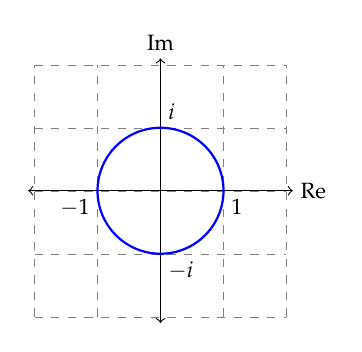
\begin{tikzpicture}[scale=.80,every node/.style={scale=0.8}]
   \draw[gray, line width=0.05mm, dashed, xstep=1, ystep=1] (-2,-2) grid (2,2);
   \draw[<->] (-2.1,0) -- (2.1,0) node[right] {$\text{Re}$};
   \draw[<->] (0,-2.1) -- (0,2.1) node[above] {$\text{Im}$};
   \draw[color=blue,thick] (0,0) circle (1);
   \node[below right] at (1,0) {$1$};
   \node[above right] at (0,1) {$i$};
   \node[below right] at (0,-1) {$-i$};
   \node[below left] at (-1,0) {$-1$};
\end{tikzpicture}
\end{center}
 \end{Solution}

 \item $\abs{z-i-1}\leq2$
 \begin{Solution}
  Let $z=x+yi$ be the standard form of a complex number. Note that 
  \[
   \abs{z-i-1}^2 = \abs{(x-1) + (y-1)i}^2  = (x-1)^2 + (y-1)^2.
  \]
Thus $z$ satisfies the inequality $\abs{z-i-1}\leq2$ if and only if $(x-1)^2 + (y-1)^2\leq 4$. The set of points satisfying $(x-1)^2 + (y-1)^2\leq 4$ form a filled-in disk centered at $(1,1)$ and having radius $2$. This can be visualized as in the following figure.
\begin{center}
    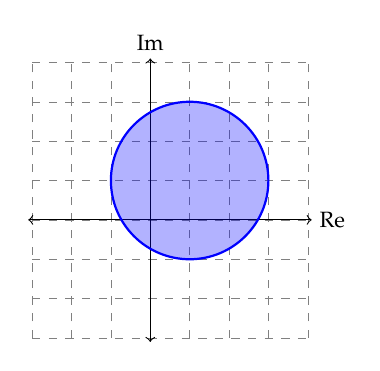
\begin{tikzpicture}[scale=.50,every node/.style={scale=0.8}]
   \draw[gray, line width=0.05mm, dashed, xstep=1, ystep=1] (-3,-3) grid (4,4);
   \draw[<->] (-3.1,0) -- (4.1,0) node[right] {$\text{Re}$};
   \draw[<->] (0,-3.1) -- (0,4.1) node[above] {$\text{Im}$};
   \draw[fill=blue,opacity=0.3] (1,1) circle (2);
   \draw[color=blue,thick] (1,1) circle (2);
   %\node[below ] at (1,0) {$1$};
   %\node[right] at (0,1) {$i$};
   %\node[right] at (0,-1) {$-i$};
   %\node[below] at (-1,0) {$-1$};
\end{tikzpicture}
\end{center}
 \end{Solution}

 \item $\abs{z-1}<\abs{z}$
 \begin{Solution}
  This inequality is equivalent to $0<\abs{z}^2-\abs{z-1}^2$. For a complex number Cartesian coordinates $z=x+yi$, note that
  \begin{align*}
   \abs{z}^2-\abs{z-1}^2 &= x^2+y^2 - \left((x-1)^2 + y^2\right)\\
			   &= 2x-1,
  \end{align*}
  and thus $z$ satisfies $0<\abs{z}^2-\abs{z-1}^2$ if and only if $0<2x-1$, or equivalently $x>\frac{1}{2}$.
Thus, the region satisfying this inequality is the region of all point that lie to the right of the line defined by the equation $x=\frac{1}{2}$. This can be visualized as in the following figure.
\begin{center}
    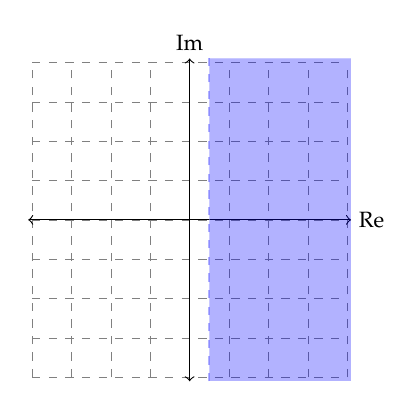
\begin{tikzpicture}[scale=.50,every node/.style={scale=0.8}]
   \draw[gray, line width=0.05mm, dashed, xstep=1, ystep=1] (-4,-4) grid (4,4);
   \draw[<->] (-4.1,0) -- (4.1,0) node[right] {$\text{Re}$};
   \draw[<->] (0,-4.1) -- (0,4.1) node[above] {$\text{Im}$};
   \draw[white,fill=blue,opacity=0.3] (.5,-4.1) rectangle (4.1,4.1);
   \draw[color=blue,thick,dashed,opacity=0.3] (.5,-4.1)--(.5,4.1);
   %\node[below ] at (1,0) {$1$};
   %\node[right] at (0,1) {$i$};
   %\node[right] at (0,-1) {$-i$};
   %\node[below] at (-1,0) {$-1$};
\end{tikzpicture}
\end{center}
 \end{Solution}

\end{enumerate}

 \item Prove for all integers $n\in\integers$ that $\operatorname{Re}((\sqrt{3}+i)^{n}) = 0$ if and only if $n\equiv 3 \pmod{6}$
\begin{Solution}
 Note that we can express $\sqrt{3}+i$ in polar form as
 \[
  \sqrt{3}+i = 2\operatorname{cis}\left(\frac{\pi}{6}\right).
 \]
 Let $n\in\integers$ be arbitrary. Using De Moivre's Theorem, we find that
 \[
  \operatorname{Re}((\sqrt{3}+i)^{n}) = \operatorname{Re}\left(\left(2\operatorname{cis}\left(\frac{\pi}{6}\right)\right)^n\right) = 2^n\operatorname{Re}\left(\operatorname{cis}\left(\frac{n\pi}{6}\right)\right) = 2^n\cos\left(\frac{n\pi}{6}\right).
 \]
Moreover, recall that $\cos(\theta)=0$ if and only if $\theta = \frac{\pi}{2} + k\pi$ for some integer $k\in\integers$. Hence,
\begin{align*}
 \operatorname{Re}((\sqrt{3}+i)^{n}) =0
    & \iff 2^n\cos\left(\frac{n\pi}{6}\right) = 0\\
    &\iff \cos\left(\frac{n\pi}{6}\right)=0\\
    &\iff \exists k\in\integers, \frac{n\pi}{6} = \frac{\pi}{2} + k\pi\\
    &\iff\exists k\in\integers, n\pi = 3\pi + 6k\pi\\
    &\iff\exists k\in\integers, n = 3 + 6k\\
    &\iff n\equiv 3\pmod{6},
\end{align*}
as desired.

 \end{Solution}
 
 \item Prove that, for all complex numbers $z\in\complex$, 
 \[
  |\operatorname{Re}(z)| + |\operatorname{Im}(z)| \leq \sqrt{2}|z|.
 \]
\begin{Solution}
 \begin{proof}
  Let $z\in\complex$ and let $x,y\in\reals$ such that $z=x+yi$. Then the real and imaginary parts of $z$ are
  \[
   \operatorname{Re}(z) = x\qquad\text{and}\qquad\operatorname{Im}(z)=y.
  \]
Now, note that $x^2 = |x|^2$ and $y^2=|y|^2$, and thus
\begin{align*}
 \left(|\operatorname{Re}(z)| + |\operatorname{Im}(z)|\right)^2 & = (|x|+|y|)^2\\
  & = |x|^2 + 2|x||y| + |y|^2\\
& \leq |x|^2 + 2|x||y| + |y|^2 + (|x|-|y|)^2 && \text{[because }0\leq (|x|-|y|)^2]\\
&=2|x|^2 + 2|y|^2 + 2|x||y| - 2|x||y|\\
& = 2(|x|^2 + |y|^2) \\
& = 2(x^2+y^2)\\
& = 2|z|^2.
\end{align*}
Hence we find that $\left(|\operatorname{Re}(z)| + |\operatorname{Im}(z)|\right)^2\leq 2|z|^2$. Taking the square root of both sides yields
\[
|\operatorname{Re}(z)| + |\operatorname{Im}(z)| \leq \sqrt{2}|z|.
\]

 \end{proof}

\end{Solution}

 
 
 \item Let $f(x) = x^3 -7x^2 +17x -15$.
 \begin{enumerate}
 \item Show that $f(2+i)=0$.
 \begin{Solution}
  Using the binomial theorem, we have
  \[
   (2+i)^3 = 2^3 + 3\cdot 2^2\cdot i + 3\cdot 2\cdot i^2 + i^3 = 8 + 12i-6-i = 2+11i
  \]
  and 
  \[
   (2+i)^2 = 2^2 + 2\cdot 2\cdot i + i^2 = 2+4i-1 = 1+4i.
  \]
Hence
\begin{align*}
 f(2+i) &= (2+i)^3 -7(2+i)^2+17(2+i)-15\\
        &=(2+11i) -7\cdot (1+4i) + 17(2+i)-15\\
        & =2+11i - 7 -28i + 24 + 17 i - 15\\
        & =(2-7+24-15) + (11-28+17)i\\
        & = 0+0i = 0.
\end{align*}


 \end{Solution}

 \item Use the fact that $2+i$ is a root of $f(x)$ to completely factor $f(x)$ in both $\complex[x]$ and $\reals[x]$.
 \begin{Solution}
  Because $2+i$ is a root of $f(x)$ and $f(x)\in\reals[x]$, we know that its conjugate $\overline{2+i}=2-i$ is also a root of $f(x)$. Hence, the polynomial
  \[
   \bigl(x-(2+i)\bigr)\bigl(x-(2-i)\bigr) = x^2-4x+5
  \]
  is a factor of $f(x)$. Performing polynomial long division, we find that
  \[
    \polylongdiv{x^3 -7x^2 +17x -15}{x^2-4x+5}
  \]
and thus $f(x)=x^3 -7x^2 +17x -15$ can be factored as
\[
 f(x)=(x^2-4x+5)(x-3).
\]
Note that $x^2-4x+5$ is irreducible in $\reals[x]$, so this is the complete factorization of $f(x)$ in $\reals[x]$. Meanwhile, the complete factorization of $f(x)$ in $\complex[x]$ is
\[
  f(x)=\bigl(x-(2+i)\bigr)\bigl(x-(2-i)\bigr)\bigl(x-3\bigr).
\]
The location of the roots in the complex plane are visualized in the figure below.
\begin{center}
    \begin{tikzpicture}[scale=.80,every node/.style={scale=0.8}]
   \draw[<->] (-5/2,0) -- (5/2,0) node[right] {$\text{Re}$};
   \draw[<->] (0,-5/2) -- (0,5/2) node[above] {$\text{Im}$};
   \filldraw [red] (-3,0) circle (2pt) node[above, black] {$-3$};
   \filldraw [red] (2,1) circle (2pt) node[above left, black] {$2+i$};
   \filldraw [red] (2,-1) circle (2pt) node[below right, black] {$2-i$};
\end{tikzpicture}
\end{center}
\end{Solution}

 \end{enumerate}
 \item Let $f(x) =x^4 - 3 x^3 + 5 x^2 - 3 x + 4$. Verify that $f(i)=0$ and use this fact to completely factorize $f(x)$ in $\reals[x]$ and $\complex[x]$.
 \begin{Solution}
  Note that $i^4=-1$, $i^3=-i$, and $i^2-1$, hence
  \[
   f(i) = 1 +3i -5 -3i +4 = 0 + 0i = 0.
  \]
Hence $i$ is a root of $f(x)$ and it follows that $-i$ is also a root of $f(x)$. Thus
\[
 (x-i)(x+i) = x^2+1
\]
is a divisor of $f(x)$. We can use polynomial long division to find that 
\[
    \polylongdiv{x^4 - 3 x^3 + 5 x^2 - 3 x + 4}{x^2+1}
  \]
and thus we can factor $f(x)$ as
\[
 f(x) = (x^2+1)(x^2-3x+4).
\]
It remains to factor $x^2-3x+4$. Note that $3^2-4\cdot 4 = 9-16 = -7 <0$, and thus this polynomial has no real roots. However, we can still use the quadratic equation to find the complex roots. The roots are of the form
\[
 x = \frac{3 \pm \sqrt{3^2-4\cdot 4}}{2} = \frac{3\pm\sqrt{-7}}{2} = \frac{3\pm i\sqrt{7}}{2}.
\]
So all of the roots of $f(x)$ are
 \[
  i,\quad -i, \quad \frac{3+ i\sqrt{7}}{2}, \quad\text{and}\quad \frac{3- i\sqrt{7}}{2}.
 \]
Hence the factorization of $f(x)$ is $\complex[x]$ is
\[
 f(x) = (x-i)(x+i) \left(x - \frac{3+ i\sqrt{7}}{2}\right)\left(x - \frac{3- i\sqrt{7}}{2}\right)
\]
while the factorization of $f(x)$ in $\reals[x]$ is
\[
 f(x) = (x^2+1)(x^2-3x+4).
\]
The location of the roots in the complex plane are visualized in the figure below.
\begin{center}
    \begin{tikzpicture}[scale=.80,every node/.style={scale=0.8}]
   \draw[<->] (-5/2,0) -- (5/2,0) node[right] {$\text{Re}$};
   \draw[<->] (0,-5/2) -- (0,5/2) node[above] {$\text{Im}$};
   \filldraw [red] (0,-1) circle (2pt) node[below left, black] {$-i$};
   \filldraw [red] (0,1) circle (2pt) node[above left, black] {$i$};
   \filldraw [red] (1.5,-1.73) circle (2pt) node[below right, black] {$\frac{3-i\sqrt{7}}{2}$};
   \filldraw [red] (1.5,1.73) circle (2pt) node[above right, black] {$\frac{3+i\sqrt{7}}{2}$};
\end{tikzpicture}
\end{center}

 \end{Solution}
 
 \item Let $z,w\in\complex$. Prove that $\abs{z+iw}=\abs{z-iw}$ if and only if $z\overline{w}\in\reals$.
 
 \begin{Solution}
  First note that $\overline{z\overline{w}} = \overline{z}w$, and so by Properties of the Conjugate (PCJ) we have
  \[
   z\overline{w} - \overline{z}w = 2i\Im(z\overline{w}).
  \]
  and thus 
  \[
   i(z\overline{w} - \overline{z}w) = -2\Im(z\overline{w}).
  \]
  Note that $\overline{iw}=-i\overline{w}$ and thus $\overline{z+iw}=\overline{z}-i\overline{w}$ by PCJ, and by the Properties of the Modulus (PM) we have
  \begin{align*}
   \abs{z+iw}^2 = (z+iw)\overline{(z+iw)} &= (z+iw)(\overline{z}-i\overline{w})\\
                                        &=z\overline{z} +i\overline{z}w-iz\overline{w} +w\overline{w}\\
                                        &=\abs{z}^2 + \abs{w}^2 -i(z\overline{w}-\overline{z}w)\\
                                        &=\abs{z}^2 + \abs{w}^2 +2\Im(z\overline{w}).
  \end{align*}
Similarly, note that $\overline{z-iw}=\overline{z}+i\overline{w}$ and thus
\begin{align*}
    \abs{z-iw}^2 = (z-iw)\overline{(z-iw)} &= (z-iw)(\overline{z}+i\overline{w})\\
                                        &=z\overline{z} -i\overline{z}w+iz\overline{w} +w\overline{w}\\
                                        &=\abs{z}^2 + \abs{w}^2 +i(z\overline{w}-\overline{z}w)\\
                                        &=\abs{z}^2 + \abs{w}^2 -2\Im(z\overline{w}).
  \end{align*}
  Hence $\abs{z+iw}=\abs{z-iw}$ is satisfied if and only if $\Im(z\overline{w}) = -\Im(z\overline{w})$ which occurs if and only if $\Im(z\overline{w})=0$, which is equivalent to $z\overline{w}\in\reals$. 
 \end{Solution}



\end{enumerate}
\end{document}
